\documentclass[a4paper,fontsize=13pt]{scrartcl}
\pagestyle{empty} % suppress page numbers

% set margins
\usepackage[left=1.0cm,top=1.0cm,right=1.0cm,bottom=1.0cm,bindingoffset=0cm]{geometry}
% \usepackage[left=0.5cm,top=0.5cm,right=0.5cm,bottom=0.5cm,bindingoffset=0cm]{geometry}

%%%%%%%%%
% fonts %
%%%%%%%%%

% use the Alegreya font
\usepackage{Alegreya}
\usepackage{AlegreyaSans}

% a times new roman clone
% \usepackage{times}

% true Times New Roman with XeLaTeX
%\usepackage{fontspec}
%\setmainfont{Times New Roman}

\usepackage[svgnames,hyperref]{xcolor}
\usepackage{url}
\usepackage{graphicx}

\usepackage{amsmath,amssymb,amsthm}
\usepackage{tikz}
\usetikzlibrary{shapes,arrows}
\usepackage[utf8]{inputenc}

\usepackage[%
backend=biber,
style=authoryear, % numeric-comp
maxbibnames=10,
url=false,
doi=false]{biblatex}

% make bibliography a bit smaller if necessary
\renewcommand*{\bibfont}{\small} 
% \footnotesize should be 10pt with a standard 12pt class, 
% see https://en.wikibooks.org/wiki/LaTeX/Fonts#Sizing_text

% \AtEveryBibitem{\clearfield{month}}
% \AtEveryCitekey{\clearfield{month}}

\addbibresource{references.bib}

\usepackage[english=british,threshold=15,thresholdtype=words]{csquotes}
\SetCiteCommand{\parencite}

\newenvironment*{smallquote}
{\quote\small}
{\endquote}
\SetBlockEnvironment{smallquote}

\usepackage[%
unicode=true,
hyperindex=true,
bookmarks=true,
colorlinks=true, % change to false for final
pdfborder=0,
allcolors=DarkBlue,
% plainpages=false,
pdfpagelabels,
hyperfootnotes=true]{hyperref}

\usepackage{todonotes}

\author{}

\date{\today}

\begin{document}

\section*{C1. Project Description}
\label{sec:project-description}
% (Please upload a Project Description as detailed in the Instructions
% to Applicants in no more than 10 A4 pages and in the required
% format. Please refer to the Instructions to Applicants for detailed
% instructions on the required content and format of the Project
% Description.)

\subsection*{PROJECT TITLE}
% can differ from grant title and be longer 

\textbf{Live and interactive parameter-space exploration of environmental simulations with uncertainty quantification}

\subsection*{AIMS AND BACKGROUND}

When systems are disrupted during environmental disasters (for example
during floods, storm surges or tsunamis) information from
computational simulation is needed urgently to aid decision-making by
emergency services. This is not simply a matter of compute power but
requires insight from computational fluid dynamics, software
engineering, human computer interaction, high performance computing
and data visualisation. All of these facets need to be tightly coupled
and tested in realistic team-coordination and decision-making
scenarios where decision-makers collaborate with modelling experts. In
particular, a crucial aspect of advice provided from modellers to
decision makers is to properly quantify and communicate the
\emph{uncertainty} in predictions obtained by computer simulations.
This advice needs to be provided in a timely manner and in a context
where the computer support may vary dramatically over time due to
system outages.

We will address this grand challenge through a \emph{live programming}
approach to the development and deployment of software systems for
environmental simulation in the presence of uncertainty. We will
develop new ``inundation models'' (models of riverine floods, storm
surges and tsunamis) which use sparse grids and uncertainty
quantification to dramatically increase the speed, quality and
usefulness of model predictions and their associated uncertainty. We
will deploy ``live'' distributed computing infrastructure to
\emph{rapidly prototype} the human interface to these new
environmental simulations and to transform the traditional,
batch-oriented workflow of environmental simulation into a highly
interactive one. We will evaluate team coordination and
decision-making in the presence of uncertainty through role-playing
scenarios of representative flood and tsunami scenarios, analysing the
protocols of live-coding optimisation of the software system during
those field trials. From these protocols, identifiable states and
transitions between those states will be used to iterate our
software-system development.

Our vision is that decision makers will be able to examine many
different environmental disaster scenarios in a short space of time,
even with computationally-expensive models. This will enable them to
develop an intuitive understanding of the uncertainty relationships in
the system---from uncertainties in input data through to
representations of uncertainty in model outputs. The importance of
this human-in-the-loop workflow is expressed
by~\textcite{pike_science_2009} in the following quote: ``it is
through the interactive manipulation of a visual interface---the
analytic discourse---that knowledge is constructed, tested, refined
and shared.''

Although the mathematical and computational tools we will employ in
this project are generalisable to any modelling workflow, our focus is
on specific application domains where (a) the model is
(computationally) complex, (b) uncertainty is significant and (c)
decisions are time-sensitive. Specifically, we will build interactive
interfaces for riverine floods, storm surge and tsunami modelling,
which exemplify these characteristics.

The mathematical component of this project will be based on new
developments combining model order reduction techniques and uncertainty
quantification. One of the main difficulties in current models is the
high dimensional spaces involved, both in the parameter and
domain spaces. Sparse grids \parencite{BungartzGriebel2004} are
well-known to reduce the effects of the so called ``curse of
dimensionality", whereby the cost of computation increases
exponentially with the dimension of the model.
We have recently found new ways to incorporate gradient
information and multi-fidelity models into sparse grid
approximations~\parencite{deBaarHarding2015,Jakeman2015,deBaarRDM2015}
and we will use this knowledge in our construction of a suite of
storm surge-tsunami models to simulate environmental disasters with
uncertainty quantification. Reduced basis 
methods~\parencite{quarteroni2015reduced} provide an alternative approach
for constructing a reduced order models and will also be investigated.

Computational decision support systems for disaster management have
existed for many decades \parencite{wallace_decision_1985}, and
advances have been made both in incorporating
uncertainty \parencite{thompson_social_2014-1,neale_navigating_2015}
and providing real-time interaction and
output~\parencite{yu_support_2006}. More recently, mixed-reality game
scenarios have been used to understand and optimise human-agent
collaboration for disaster response~\parencite{ramchurn2016human}. In
our project plan we will follow a similar approach and will employ
mock-game scenarios to examine and understand the nature of decision
making with expert modelling support. In a novel twist, we will run
these games together with live-coding optimisation and tuning of the
software system and the underlying computational platform. By
analysing the protocols of these live optimisations, we will
accumulate data to feed into redesign of the software interface and to
understand the time requirements and controls needed for the
computational platform.


This project will provide the following discoveries and benefits:
\begin{enumerate}

\item a suite of interactive, real-time modelling tools for
  surge-tsunami flood disasters which combine high fidelity
  simulations (fine grids) with low fidelity (coarse grid) simulations
  to quantify uncertainty, optimised for human exploration

\item a ``live software engineering'' approach to the development,
  deployment and optimisation of these interactive software systems;

\item models of group interaction scenarios for decision-making with
  expert modelling support; from these models, empirical estimates of
  the time constraints that such scenarios impose on software
  and computer system requirements and the live controls needed to run
  them effectively in volatile contexts

\item interactive information visualisation of simulation predictions
together with uncertainties
 

\end{enumerate}

This research is significant because it aims to unlock the power of
sophisticated computational simulation for \emph{interactive} use.
Although we concentrate our research on simulation support for
disaster response, the ultimate potential of this work is to
eventually empower domain experts from a broad range of areas to
better use the high-performance computing power which is now available
to them. We envision a future where performing a complex flood model
or disaster simulation is as interactive and \emph{alive} as flicking
through photos on an iPad.

\subsection*{RESEARCH PROJECT}
% - Describe how the research is significant and how it addresses an important problem
% - Describe how the Proposal meets the objectives of the Discovery Projects scheme
% - Describe how the anticipated outcomes will advance the knowledge base of the discipline and
%   how the Proposal aims and concepts are novel and innovative
% - Outline the conceptual framework, design and methods and demonstrate that these are
%   adequately developed, well integrated and appropriate to the aims of the Proposal. Include
%   research plans and proposed timelines
% - Detail what new methodologies or technologies will be developed in the course of the research
%   and how they will advance knowledge
% - Outline the feasibility of the project, in terms of design, budget and proposed timeline
% - If the rationale for some of the Proposal rests upon manuscripts that are still in the process of
%   being published, or on results of work that may not be available to assessors, include a
%   summary of the relevant work
% - Describe the expected outcomes and likely impact of the proposed research
% - Describe how the Proposal might result in national or international economic, commercial,
%   environmental, social and/or cultural benefits
% - If the research has been nominated as focussing upon a topic or outcome that falls within one
%   of the Science and Research Priorities, describe the potential for the project to contribute to the associated Priority Goals.

The January 2011 Brisbane River floods in south-east Queensland cost
32 lives and caused 2.5~billion dollars worth of
damage~\parencite{vandenhonert_2011_2011}. In the days leading up to
these events, a key issue facing authorities was incorporating their
\textbf{uncertainty} about the preceding fortnight's rainfall into the
modelling. In their report on the causes, impacts and implications of
the floods, \textcite[p1170]{vandenhonert_2011_2011} concluded:
\blockquote{whilst the dam operators were acting in accordance with
  the operations manual for the dam, their modelling did not take
  account of forecast rainfall in determining the predicted dam water
  level, and this resulted in a sub-optimal water release strategy.
  Employing tools for decision making under uncertainty would have
  resulted in a different water release strategy.} At the other end of
the environmental spectrum, bushfire model predictions are similarly
\textquote[\cite{alexander_limitations_2013} p375]{fraught with
  uncertainty}. As Australia's climate changes and extreme weather
events become more common, there is a significant need for better ways
to gather timely insights from modelling in the presence of
uncertainty and to communicate those insights to decision makers and
emergency services.

Computational modelling and simulation is an invaluable support tool
for disaster response, allowing emergency services personnel to
explore what might happen in the immediate future under various
scenarios. But these model simulations can be fraught with
uncertainty: some of their \emph{input parameters} may be well known
(possibly from reliable sensor data), others may be known only
approximately, and others still may only be guessed at. Even with
perfect input data, the models themselves entail assumptions and
numerical approximations which bound the reliability of their
predictions.

More formally, suppose that we have a mathematical model
$M_{\mathbf{p}}$ parameterised by the vector
$\mathbf{p}\in\mathcal{P}$. For example, $M_{\mathbf{p}}$ may be a
parameterised partial differential equation %(PPDE)
in a storm surge model. For each $\mathbf{p}$ we suppose the model is
well-defined and there exists a unique function
\begin{equation}
  \label{eq:1}
  u_{\mathbf{p}}(\mathbf{x})\, \quad \mathbf{x}\in\Omega
\end{equation}
which is a solution to the model problem, that is $M_{\mathbf{p}}(u_{\mathbf{p}})=0$.
Here the \emph{domain space} $\Omega$ represents variables such as 
time and space, 
and $u_{\mathbf{p}}$ represents scalar or vector fields of interest, 
such as storm surge water level and/or velocity.    

Sometimes the goal of the modeller is to better understand the
relationship between $\mathbf{p}$ and some lower-dimensional quantity
of interest $Q(u_{\mathbf{p}})$, such as the relationship between a
particular rainfall scenario and the maximum storm surge levels at
particular geographical locations. In order to achieve such
understanding, repeated executions of the model are often required
with an expert analysis of the outputs of each stage and selection of
the next parameter set based on an assessment of those outputs. Such
repeated model executions can also be used to estimate the
\emph{uncertainty} in any given set of predictions of
$Q(u_{\mathbf{p}})$. Through the process of trying different model
parameterisations, the scientist is able to build up an understanding
of the \emph{general} relationship between $\mathbf{p}$ and
$Q(u_{\mathbf{p}})$, including the areas of the parameter space
$\mathcal{P}$ which have the greatest influence on the result and
which types of uncertainty have the greatest impact on the certainty
of the results.

%or to find the parameter choice $\mathbf{p}$
%which optimises $Q$. %over all $\mathbf{x}$.
%This high-level description of the ``model selection/optimisation''
% workflow 
%(shown
%graphically in Figure~\ref{fig:general-fb-loop})
 %lies at the heart of
%a great deal of modern science.
%\begin{figure}
 % \centering
  %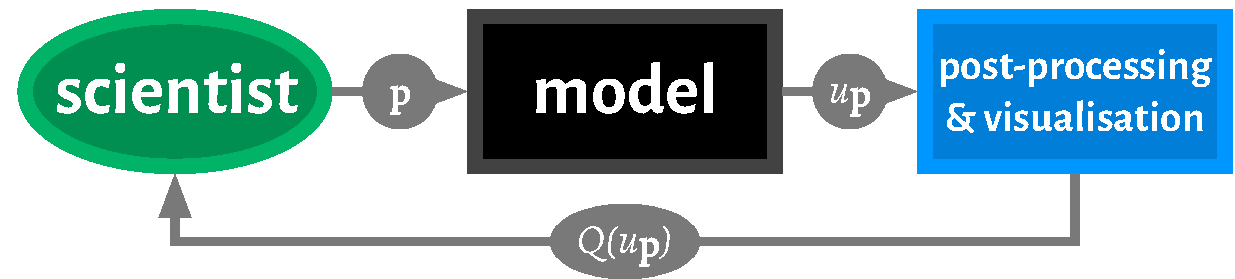
\includegraphics[width=.6\textwidth]{figures/general-fb-loop.pdf}
  %\caption{The human-in-the-loop modelling workflow. A scientist
    %selects an initial parameter $\mathbf{p_0}$ for their model,
    %examines the model output $Q(u_{\mathbf{p}})$, and either accepts
    %the output of the model or re-runs the model with a different
    %choice of the parameter $\mathbf{p_1}$.}
  %\label{fig:general-fb-loop}
%\end{figure}
%There are many ways of finding an optimal $\mathbf{p}$, from 
%trial-and-error experimentation to expert judgement through to fully-automated algorithmic
%optimization procedures. Often there are ways to optimise $\mathbf{p}$
%algorithmically, although these methods often introduce new parameters (the
%arguments of the function being optimised) which must be selected by the
%scientist. 
%As a result, this feedback loop will often require many
%iterations, with a scientist-in-the-loop, evaluating the results
%of the model (possibly through visualising the model output) and
%choosing a parameter update $\Delta\mathbf{p}$ at each step.
% (see
%Figure~\ref{fig:unrolled-fb-loop}). 
%Each step through this loop
%provides feedback to the scientist about the response of the system to
%a particular value of $\mathbf{p}$ --  for example, the maximum storm
%surge level under a particular rainfall scenario. 

%\begin{figure}
% \centering
%  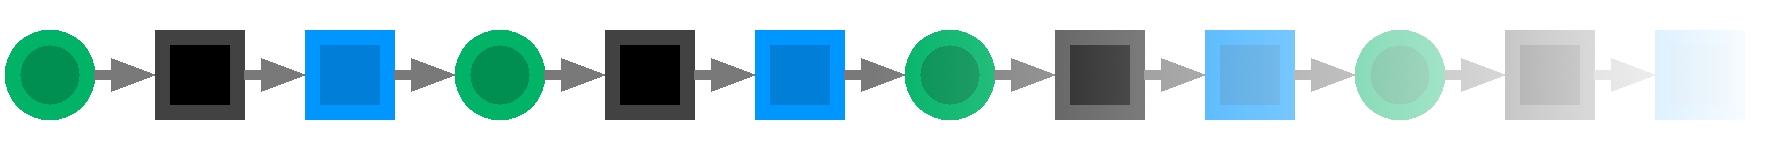
\includegraphics[width=\textwidth]{figures/unrolled-fb-loop.pdf}
%  \caption{If the modelling \& post-processing/visualisation steps can
%    be performed sufficiently quickly, then the scientist can explore
%    the $\mathbf{p} \rightarrow Q(u_{\mathbf{p}})$ relationship
%    \emph{interactively}, with the all the associated benefits for
%    exploratory analysis.}
%  \label{fig:unrolled-fb-loop}
%\end{figure}

From a workflow perspective, the productivity of the
modeller/scientist is proportional to the rate at which they can
explore the $\mathbf{p} \rightarrow Q(u_{\mathbf{p}})$ relationship.
Any latency improvements in this feedback loop will translate into
productivity gains~\parencite{liu_effects_2014}. If the model
parameters $\mathbf{p}$ and inputs $\mathbf{x}$ are known precisely
and the quantity $Q(u_{\mathbf{p}})$ is cheap to calculate and easy to
interpret, then the task is simple: provide the scientist with an
interface for manipulating $\mathbf{p}$ and set them loose. However,
for real-world models (such as those used in flood/storm
surge/bushfire modelling) this is often not the case. There are
\textbf{three primary challenges}:
\begin{enumerate}
\item \emph{The model may not provide a way to express uncertainty in
    the inputs}. Many models do not provide methods for including
  uncertainty information in their inputs, as was the case in the 2011
  Brisbane River flood example.
\item \emph{The quantity $Q(u_{\mathbf{p}})$ may not be cheap to
    calculate}. Many
  sophisticated models require non-trivial computing resources to evaluate. These compute resources may be
  difficult to secure, with submitted jobs having to wait in a queue, and may
  take a long time to compute even when the resources are available.
  This is especially problematic in a disaster-response scenario,
  where an approximately correct answer provided in a short time is
  significantly more useful than a perfect answer provided after it is
  too late to act on.
\item \emph{The quantity $Q(u_{\mathbf{p}})$ together with estimates
    of its uncertainty may not be easy to interpret}. Oftentimes this
  is a visualisation problem--- the mapping
  $\mathbf{p} \rightarrow Q(u_{\mathbf{p}})$ may be high-dimensional,
  and presenting that to a decision-maker, particularly when combining
  it with its uncertainty estimates, may not be straightforward.
\end{enumerate}
%\begin{figure}
 % \centering
  %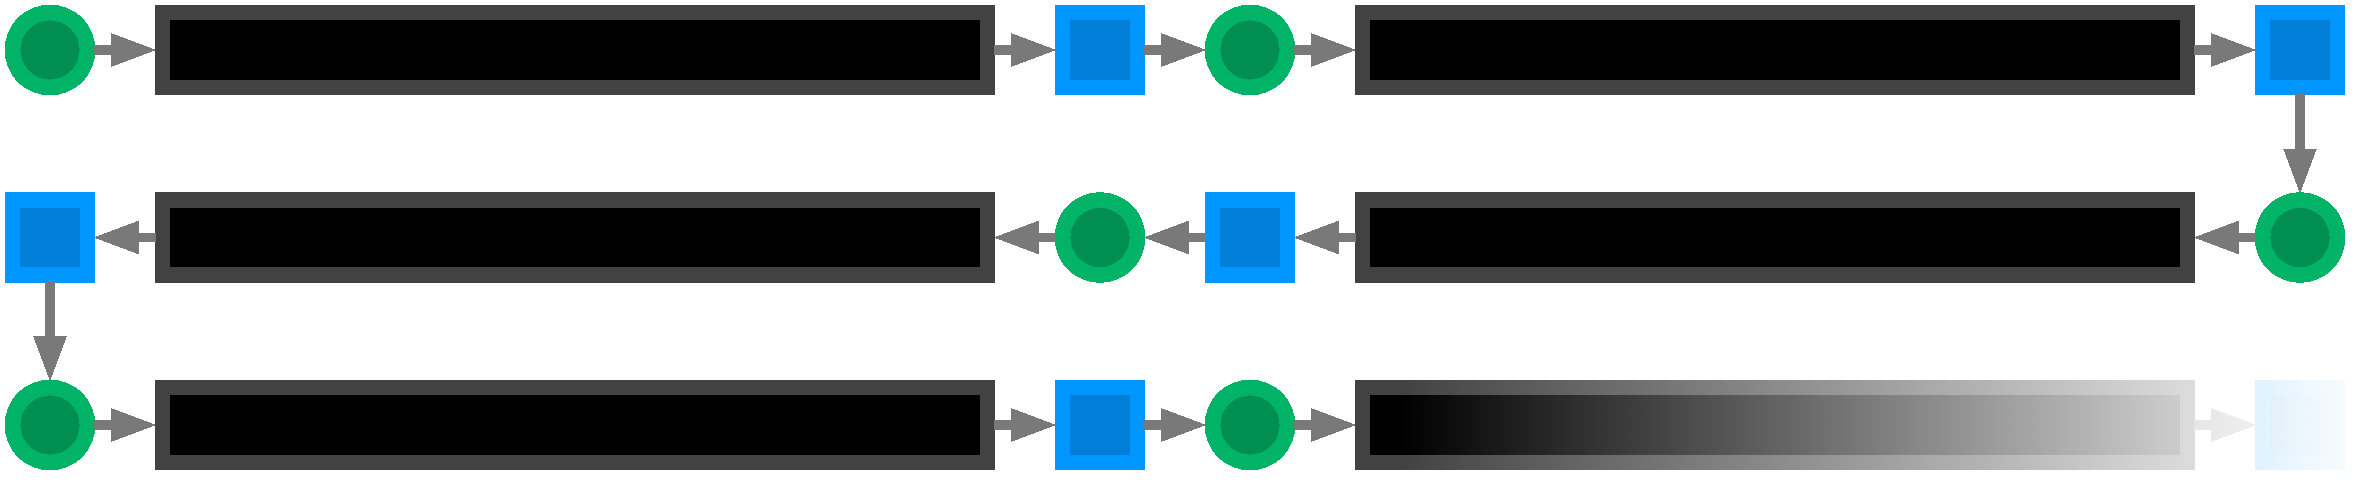
\includegraphics[width=\textwidth]{figures/long-fb-loop.pdf}
  %\caption{If the model is computationally expensive to run, then the
   % workflow is dominated by waiting for the model to finish. This
    %results in lower productivity---not only due to the time spent
    %waiting for the model, but also because of the temporal separation
  %between the selection of a new parameter $\mathbf{p}$, and seeing
 % its impact on the results of the model.}
 % \label{fig:long-fb-loop.pdf}
%\end{figure}

In this project, by accelerating the feedback loop between
$\mathbf{p}$ and $Q(u_{\mathbf{p}})$, together with estimates of its
uncertainty, we will give the scientist the ability to interactively
\emph{explore} the connection (and the associated uncertainty) between
the different dimensions of $\mathbf{p}$ and the overall response of
the system. By understanding the human-factors and systems-level time
constraints on the delivery of useful information in disaster-response
settings, we will be able to specify timing requirements on our model
simulations. By developing software that is time-constrained and
time-aware, we will be able to provide decision makers with
information when it is needed and with an estimate on the uncertainty
of that information.

%Ultimately, the scientist needs an \textbf{interactive interface} for
%gleaning insights from their models in the presence of these
%challenges.

We will address these three challenges using sparse grids and reduced
basis models combined with live modification of simulation parameters,
dynamic steering of computational resources and interactive
visualisation. Specifically:
\begin{enumerate}
\item \emph{Uncertainty in inputs:} sparse grids and reduced basis models can be used
  to precompute a surrogate model, $\mathbf{p} \rightarrow \tilde{u}_{\mathbf{p}}$, of the original
  (expensive) model solution process, $\mathbf{p} \rightarrow {u}_{\mathbf{p}}$.
  The expectation integrals of the original model over subsets of the
  parameter space $\mathcal{P}$ (which are important for quantifying
  uncertainty) can be efficiently estimated from the
  surrogate model. This has
  significant benefits over classical Monte Carlo methods when the
  integrand is sufficiently
  smooth~\parencite{JakemanRoberts2013,FranzelinDiehlPfluger2014}.

\item \emph{Cheap to calculate:} for many problems the computation
  of solutions $u_{\mathbf{p}}(\mathbf{x})$ to the model
  $M_{\mathbf{p}}$ can be done cheaply using the combination technique
  over the domain $\mathbf{x}\in\Omega$. An alternative is to use
  proper orthogonal decompositions or greedy algorithms to construct a
  reduced order model which is then cheap to compute with. In both
  cases the initial construction can be somewhat costly but the
  savings gained later when these surrogates are used extensively for
  UQ and optimisation significantly outweight this cost. Additionally,
  the initial construction can be done in an offline phase. For our
  disaster response scenarios, the concept of ``cheapness'' will be
  reframed as one of ``timeliness'': we will build systems which
  guarantee modelling results within particular timeframes of
  relevance to human factor processes in group decision making
  (occurring in the online phase).

\item \emph{Easy to interpret:} since a sparse grid sampling of
  $\mathbf{p}\in\mathcal{P}$ enables a fast and efficient exploration
  of parameter space, there is more time for visualisation and
  post-processing in an interactive interface, which facilitates
  richer ensembles of visualisation techniques to assist the
  decision-maker in interpreting the results of the model.
\end{enumerate}

%\begin{figure}
 % \centering
  %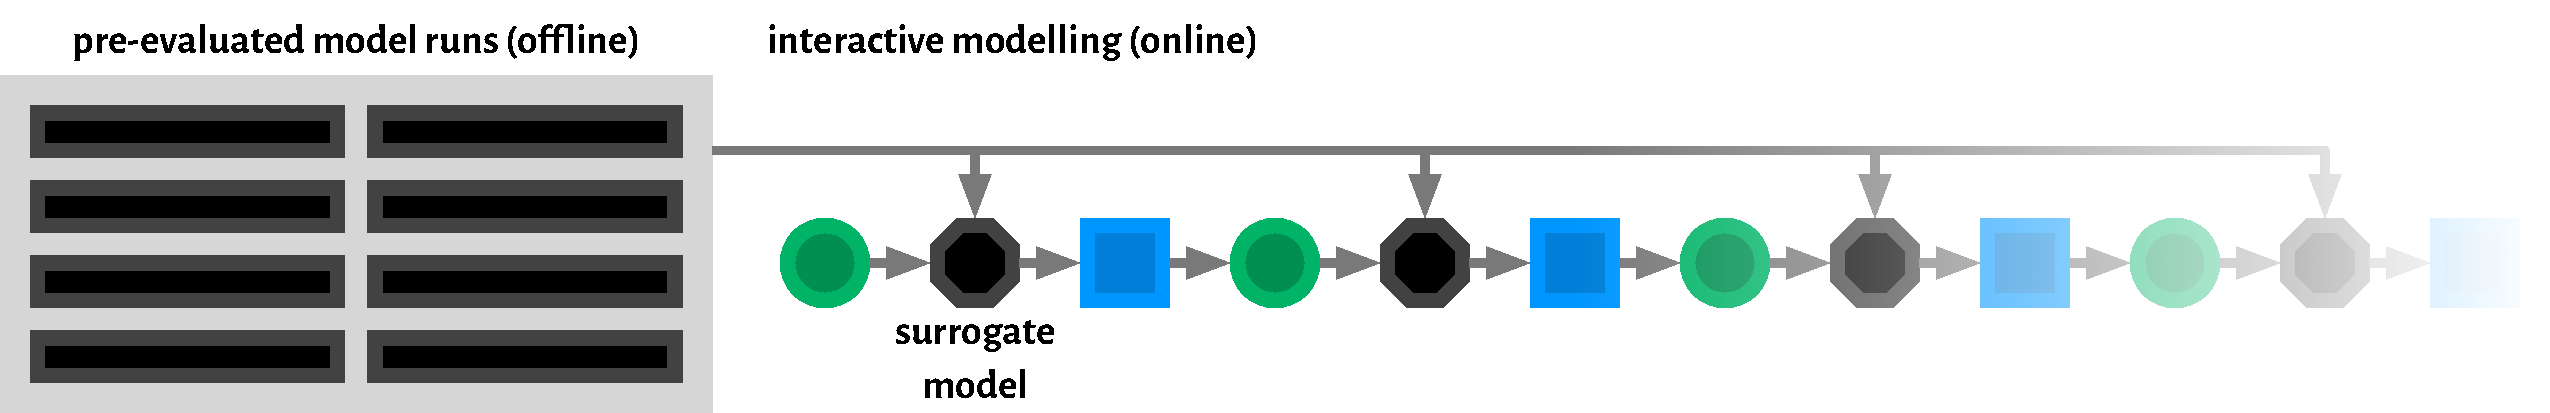
\includegraphics[width=\textwidth]{figures/sg-surrogate-model-fb-loop.pdf}
  %\caption{Using the sparse grids and reduced basis models, the computationally
   % expensive model calculations can be done ahead-of-time and used to
    %construct a surrogate model which can be used to re-claim the
    %interactive workflow of Figure~\ref{fig:unrolled-fb-loop}}.
  %\label{fig:sg-surrogate-model-fb-loop}
%\end{figure}

%Impact: new algorithms, software, high performance computer systems
%and visualisation techniques for time-bound environmental simulation
%with uncertainty. New software tools for the simulation of flood
%surges and tsunami. New methodologies for rapid and agile software
%development and usability using live programming. New knowledge of
%human-in-the-loop requirements for support systems in the context of
%environmental disaster management. New algorithms, software, high
%performance computer systems and visualisation techniques for
%time-bound environmental simulation with uncertainty. New software
%tools for the simulation of flood surges and tsunami. New
%methodologies for rapid and agile software development and usability
%using live programming. New knowledge of human-in-the-loop
%requirements for support systems in the context of environmental
%disaster management.





\subsubsection*{Sparse-Grids and Uncertainty Quantification}

The mathematical component of this project will be based on new
developments combining sparse
grids~\parencite{BungartzGriebel2004}, reduced basis
methods~\parencite{LiebermanEtal2010,Peherstorfer2013,ChenSchwab2015,PeherstorferWillcox2015}
and uncertainty quantification. One of the main difficulties in the
study of current scientific models is the high dimensional spaces
involved, often both in the parameter and domain spaces, $\mathcal{P}$
and $\Omega$ respectively. This is a significant barrier for the
timely evaluation of models due to the ``curse of dimensionality'' in
which the cost scales exponentially with dimension. By using sparse
grids and reduced basis models we will be able to compute
\emph{surrogates of the full problem} which have significantly fewer
unkowns and are thus cheaper to compute whilst maintaining a high
order of accuracy. For example, a general approach would be to find a
lower dimensional manifold of the parameter space
$\mathcal{Q}\subset\mathcal{P}$ over which the model is most sensitive
using a proper orthogonal decomposition. A sparse grid surrogate of
the model over $\mathcal{Q}$ can also be computed in an offline phase,
so that in an online phase model solutions can be efficiently
estimated using the surrogate model. For many problems sparse grids
can also be used over $\Omega$ when computing solutions to the full
model to speed up the construction of a reduced basis. We will compute
sparse grid solutions via the ``combination
technique''~\parencite{Griebel1990}. Figure~\ref{fig:sparse_grids}
depicts the combination technique, the equivalent sparse grid and the
corresponding full grid.

\begin{figure}
  \centering
  % Brendan: combination grid, sparse grid, fullgrid figure

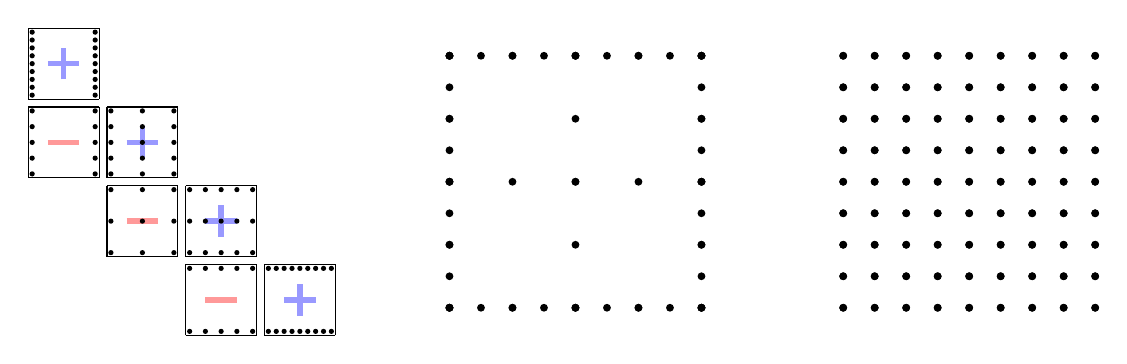
\begin{tikzpicture}%[scale=0.8]
%\scriptsize
%%% Draw squares around component grids
\foreach \i in {1,...,4}
{
	\pgfmathtruncatemacro{\x}{(\i - 1)};
	\draw[] (0.05+1.0*\x, 3.05-1.0*\x) -- (0.05+1.0*\x+0.9, 3.05-1.0*\x) {};
	\draw[] (0.05+1.0*\x, 3.05-1.0*\x) -- (0.05+1.0*\x, 3.05-1.0*\x+0.9) {};
	\draw[] (0.05+1.0*\x+0.9, 3.05-1.0*\x) -- (0.05+1.0*\x+0.9, 3.05-1.0*\x+0.9) {};
	\draw[] (0.05+1.0*\x, 3.05-1.0*\x+0.9) -- (0.05+1.0*\x+0.9, 3.05-1.0*\x+0.9) {};
	%%% optional plotting of coefficients
	\draw[blue!40,line width=0.7mm] (0.5+1.0*\x-0.2, 3.0+0.5-1.0*\x) -- (0.5+1.0*\x+0.2, 3.0+0.5-1.0*\x);
	\draw[blue!40,line width=0.7mm] (0.5+1.0*\x, 3.0+0.5-1.0*\x-0.2) -- (0.5+1.0*\x, 3.0+0.5-1.0*\x+0.2);
}
\foreach \i in {1,...,3}
{
	\pgfmathtruncatemacro{\x}{(\i - 1)};
	\draw[] (0.05+1.0*\x, 2.05-1.0*\x) -- (0.05+1.0*\x+0.9, 2.05-1.0*\x) {};
	\draw[] (0.05+1.0*\x, 2.05-1.0*\x) -- (0.05+1.0*\x, 2.05-1.0*\x+0.9) {};
	\draw[] (0.05+1.0*\x+0.9, 2.05-1.0*\x) -- (0.05+1.0*\x+0.9, 2.05-1.0*\x+0.9) {};
	\draw[] (0.05+1.0*\x, 2.05-1.0*\x+0.9) -- (0.05+1.0*\x+0.9, 2.05-1.0*\x+0.9) {};
	%%% optional plotting of coefficients
	\draw[red!40,line width=0.7mm] (0.5+1.0*\x-0.2, 2.0+0.5-1.0*\x) -- (0.5+1.0*\x+0.2, 2.0+0.5-1.0*\x);
}
%%% Combination grids
\foreach \i in {1,...,18} %2*9
{
	\pgfmathtruncatemacro{\y}{(\i - 1) / 2};
	\pgfmathtruncatemacro{\x}{\i - 1 - 2 * \y};
	\node[fill,circle,scale=0.2] at (0.1+0.8*\x,3.1+0.1*\y) {};
	\node[fill,circle,scale=0.2] at (3.1+0.1*\y,0.1+0.8*\x) {};
}
\foreach \i in {1,...,15} %3*5
{
	\pgfmathtruncatemacro{\y}{(\i-1)/3};
	\pgfmathtruncatemacro{\x}{\i-1-3*\y};
	\node[fill,circle,scale=0.2] at (1.1+0.4*\x,2.1+0.2*\y) {};
	\node[fill,circle,scale=0.2] at (2.1+0.2*\y,1.1+0.4*\x) {};
}
\foreach \i in {1,...,10} %2*5
{
	\pgfmathtruncatemacro{\y}{(\i-1)/2};
	\pgfmathtruncatemacro{\x}{\i-1-2*\y};
	\node[fill,circle,scale=0.2] at (0.1+0.8*\x,2.1+0.2*\y) {};
	\node[fill,circle,scale=0.2] at (2.1+0.2*\y,0.1+0.8*\x) {};
}
\foreach \i in {1,...,9} %3*3
{
	\pgfmathtruncatemacro{\y}{(\i - 1) / 3};
	\pgfmathtruncatemacro{\x}{\i - 1 - 3 * \y};
	\node[fill,circle,scale=0.2] at (1.1+0.4*\x,1.1+0.4*\y) {};
}
%%% Sparse grid
\foreach \i in {1,...,18} %2*9
{
	\pgfmathtruncatemacro{\y}{(\i - 1) / 2};
	\pgfmathtruncatemacro{\x}{\i - 1 - 2 * \y};
	\node[fill,circle,scale=0.3] at (5.4+3.2*\x,0.4+0.4*\y) {};
	\node[fill,circle,scale=0.3] at (5.4+0.4*\y,0.4+3.2*\x) {};
}
\foreach \i in {1,...,15} %3*5
{
	\pgfmathtruncatemacro{\y}{(\i-1)/3};
	\pgfmathtruncatemacro{\x}{\i-1-3*\y};
	\node[fill,circle,scale=0.3] at (5.4+1.6*\x,0.4+0.8*\y) {};
	\node[fill,circle,scale=0.3] at (5.4+0.8*\y,0.4+1.6*\x) {};
}
%%% Full grid
\foreach \i in {1,...,81} %9*9
{
	\pgfmathtruncatemacro{\y}{(\i - 1) / 9};
	\pgfmathtruncatemacro{\x}{\i - 1 - 9 * \y};
	\node[fill,circle,scale=0.3] at (10.4+0.4*\x,0.4+0.4*\y) {};
	\node[fill,circle,scale=0.3] at (10.4+0.4*\y,0.4+0.4*\x) {};
}
\end{tikzpicture}  
  \caption{Combination grids on the left (with coefficients, marked with
    a blue plus for $+1$ and red minus for $-1$), sparse grid in the
    middle, full grid on the right. Note the marked reduction in the number of 
    grid points for the sparse grid relative to the full grid. 
   This is even more pronounced in hgher dimensions.}
  \label{fig:sparse_grids}
\end{figure}

Propagating uncertainty in scientific models which are high
dimensional and/or expensive to compute is a significant challenge.
For models which are not stochastic in nature, and thus have no means
of directly quantifying uncertainty, one must typically estimate
statistical moments via monte carlo methods or quadrature rules. For
high dimensional problems it has been shown that sparse grids can
estimate these moments faster and more accurately than traditional
Monte Carlo methods when the probability density functions are
sufficiently
smooth~\parencite{JakemanRoberts2013,FranzelinDiehlPfluger2014}.
Despite the advantages of reduced basis methods, the manifold
$\mathcal{Q}$ is still sufficiently high dimensional that the
quantification of uncertainty remains a challenge due to the sheer
number of function evaluations required. This is particularly true
when the quantification of uncertainty in a model is a component of an
optimisation algorithm. As such it is important to continue to
developing efficient numerical methods for uncertainty quantification
for high dimensional problems. Replacing the full model with a reduced
basis model also adds additional error and uncertainties. One needs to
have some idea what the model outcomes may be for parameters not lying
on the lower dimensional manifold $\mathcal{Q}$. An important part of
developing reduced models is `verifying' the model, by bounding their
error of the surrogate for example. By using ensemble methods,
multifidelity models~\parencite{NgWillcox2014} and gradient enhanced
approximation~\parencite{deBaarHarding2015,Jakeman2015} we hope to
improve the verification and propogation of uncertainties in models.
Incorporating ideas from ``Kriging'' (Gaussian process regression), a
feature of which is having confidence intervals over an interpolant,
together with sparse-grid interpolation, we will be able to express
uncertainties explicitly in the surrogate model.


\subsubsection*{Live-Coding of Scientific Simulation}

Live coding is a term which has been used to denote systems which
support the direct intervention of the programmer in a program's
run-time state. It can be thought of as an extreme version of the
agile programming methodology~\parencite{fowler_agile_2001}, where
code changes are hot-swapped in to running programs, allowing for
extremely fast exploration and iteration of new ideas and system
updates. As the ambition of live-coding has grown, support systems and
languages have evolved to, for example, create, modify and interact
with music and hardware devices in real time. Such an approach has
been termed ``\emph{with-time}
programming''~\parencite{sorensen2010programming}. This project will
make use of the \emph{Extempore} software
environment\footnote{\url{http://extempore.moso.com.au}} which has
been shown to be able to harness a traditional batch-mode scientific
simulations, written in the C language, and visualise and modify that
simulation interactively, and in real-time, with negligible
performance overhead~\cite{swift_live_2016}. This software environment
will be a key tool for this project as it will allow us to fine tune
our suite of simulation software for disaster response scenarios.

Uncertainty quantification can benfit greatly from live coding. Specifically, the
ability to alter function sampling in real time as computations progress
has the potential to significantly improve the efficiency of an uncertainty analysis.
Indeed, there exist many algorithms, adaptive MCMC for example, which attempt to 
choose the best samples based on the sampling history. 
For complex problems however, a domain expert may often have a better idea
on where the most function evaluations should be spent.
Through live programming the domain experts input can be compared with the 
current algorithms strategy to potentially guide the next step.
The resulting strategies are expected to be more aggressive in nature as they 
are more specific to the problem at hand.


\subsubsection*{From Disaster-Response Human-Factors Optimisation to Software Development}

% GOMS model for co-operative scenarios where someone wants
% information, and someone is trying to present it to them

% it's about chunking complex tasks c.f. beginning-middle-end

% the goal: quantitative requirements on the time bounds, which has
% implications for the design of the systems

Similar to ~\parencite{ramchurn2016human} we will employ game
scenarios to understand and optimise collaboration for disaster
response~\parencite{ramchurn2016human}. However, our focus will be on
decision-maker/modeller communication rather than human/agent
communication and our game scenarios will take place while software
and systems parameters, particularly the human-computer interface,
visualisations and system configuration, are being tuned in real time
by a live coder. In a novel approach, the protocols obtained from this
live coding will then be analyse to determine macro, ``chunking''
states, of human action and transitions between those states. We have
recently used similar approaches to understand the real-time actions
of single live-coders in computer music
performance~\parencite{swift2014coding} and the macro-gesture states
of group computer musicians using
iPads~\parencite{martin2015tracking}. In both of these studies,
transition matrices derived from interaction protocols were able to
yield insights into the artistic process. In the case of the present
project, data from the interaction protocols of the live-coder will be
feed back into redesign of the software interface and the controls
needed for the computational platform.

By way of one simple example, we imagine that, perhaps, the live coder
finds that a particular measure of uncertainty, \emph{measure-A}, is
routinely requested by a decision maker after another particular
measure, \emph{measure-B}. The live coder could tune up the software
in real time so that these two measures could be presented together.
The interaction protocols in this instance might reveal insights into
the \emph{context} where these two measures were requested one after
the other and the software might be redesigned to recognise that
context and to make the two measures accessible in that context. For
another simple example, the live-coding protocol might show that data
processing needed to be occasionally shifted from one part of a cloud
resource to a local cluster. Examination of these instances could
impact on the computer systems settings needed to properly deploy
these simulations. Our approach to protocol analysis will go well
beyond simple examples like these and will use matrix theory to derive
insights into the nature of state transitions across entire protocols
and across test participants.


\subsubsection*{High-Performance Computing Systems Support}

A reliance on high performance computing for the evaluation of
scientific models provides additional challenges to the technical side
of the project. Specifically, our algorithms must be highly scalable
and robust to errors and faults in the computer system layer. There
have been many recent developments in both highly-scalable algorithms
and the sparse grid combination technique which will be of use for
this and, additionally, it has been recently shown that such
computations can be made
robust~\parencite{HardingHLS2015,AliEtal2015}. By leveraging and
continuing to develop these algorithms we can ensure that the
components of our software system that require high performance
computing resources will be both scalable and robust.

In this project we will leverage on-demand compute resources, such as
the Amazon AWS cloud~\parencite{amazon_aws} and the National Compute
Infrastructure NCI Cloud~\parencite{nci_cloud}. Using these cloud
services will further improve the project's ability to deliver timely
results in high-pressure and time-critical decision making scenarios.

Once again, we emphasise that our approach to live-coding of test
software is a novel aspect of our methodology. The \emph{Extempore}
tool that we have developed has been shown to be able to harness and
steer scientific simulation in real time. In this part of the project,
we will apply this tool to the real-time steering of the computer
systems layer itself.


\subsubsection*{Interactive visualisation of environmental forecasts with uncertainty}

Similar to the impact of visually presented geodata on decision
making~\parencite{kinkeldey2015evaluating}, the particular
visualisations of uncertainty in our environmental models will need to
be systematically evaluated with human participants. Here we will
adopt traditional human-factors trials with non-expert participants
together with qualitative feedback from emergency services experts. We
will solicit qualitative feedback from expert participants from
emergency authorities in our local area including ACT Emergency
Service, Geosciences Australia, the Australian Maritime and Safety
Authority and the Australian Federal Police. Perspectives offered by
this participant pool will be important in extrapolating our study
results to real world disaster-management.




\subsection*{ROLE OF PERSONNEL}
% - Summarise the role, responsibilities and contributions of each Chief Investigator (CI) and Partner Investigator (PI)
% - Summarise the roles and levels of involvement of other Participants, for example, technical staff, Research Associates and other personnel
% - Describe how each Participant will ensure they have the ‘time and capacity’ to undertake the proposed research, taking into account any other grants or roles that they hold.

%The personnel on this grant cover the key research areas discussed in
%the \emph{Research Project} section of this application:
%
%\begin{itemize}
%\item \textbf{Steve Roberts}: uncertainty quantification, sparse grids, flood
%  modelling
%\item \textbf{Markus Hegland}: sparse grids
%\item \textbf{Peter Strazdins}: sparse grids, distributed computing
%\item \textbf{Henry Gardner}: HCI, interfaces
%\end{itemize}

% Brendan: to some extent I have copied/reworked this section from the linkage project with Fujitsu

The personnel involved in this project will be CIs Gardner and
Roberts, two Postdoctoral Research Associates and two PhD students.
This project is split between the ANU Research School of Computer
Science (CI Gardner, one PDRA, one PhD student) and the ANU
Mathematical Sciences Institute (CI Roberts, one PDRA and one PhD
student). In addition, we forecast that upwards of four Honours
students will work with this project team over the three years of the
project.

CI Henry Gardner will be responsible for the overall project and will
lead the interactive computing and visual interface components. The
distributed computing and mathematical component will be lead by CI
Stephen Roberts. One post-doctoral fellow, to be situated in the
Research School of Computer Science (RSCS), will develop large
portions of the live programming tools and software interface which
will interact with the scientific models and will conduct experiments
on live scenarios where human actors mimic the interactions and
information flows involved in the group dynamics of disaster response
with simulation support. The second post-doctoral fellow, to be
situated in the Mathematical Sciences Institute (MSI), will develop
the numerical methods for computing sparse grid surrogates and reduced
basis models which are able to efficiently propagate uncertainties in
model applications of tsunami and flood surge events. Because of the
larger skill set and responsibilities of the computer science PDRA,
this position has been factored into the budget at a higher academic
level (B3) than the mathematics PDRA (B1). Without prejudicing a
competitive selection process, suitable candidates are known to be
available for both positions.

The two  PhD students will be split between the two departments---one
in RSCS and one in MSI, focusing on specific aspects of the project.
In RSCS, these will be the dynamic distributed computing
infrastructure and the development of live interfaces for data
visualisation. In the MSI, these will be the uncertainty
quantification and the development of numerical methods for the sparse
grid technique. We anticipate being able to support a number of Honours level projects in computer science and mathematics during the course of this project. Some of these projects will relate to the core mission of the project detailed above, others will concentrate on related studies with a view to achieving high-impact pure and applied research and training young people for a career in the computing and mathematical modelling disciplines.

\subsection*{RESEARCH ENVIRONMENT}
% - Outline the adequacy and opportunities within the Research Environment in your relevant department, school or research group, and the extent to which it will provide for knowledge growth, innovation, collaboration, mentoring and student training
% - Describe the existing, or developing, research environment within the Administering Organisation and collaborating Organisation(s) which will enable this Project
% - Describe how the Project aligns with the Administering Organisation’s research plans and strategies.

The Australian National University is a research-intensive university
of high international standing. The quality of the research at ANU has
been reflected in every one of the ERA evaluation exercises where,
relevant to the current proposal, both Information and Computing
Sciences (08) and Mathematical Sciences (01) have been assessed as
being at the highest level of 5. At ANU, the Research School of
Computer Science and the Mathematical Sciences Institute have a long
and deep collaboration in numerical and applied mathematics, notably
in a number of ''Area'' projects linked to the supercomputing
facilities on campus. Indeed, since the early 1980s ANU has housed the
largest supercomputers in Australia and the present National
Computational Infrastructure is located on campus.

Over the next 2 years, a new building will be constructed at ANU to
locate the Mathematical Sciences Institute with part of the Research
School of Computer Science. This co-location of academics in these two
areas will be particularly fruitful for the present project. Indeed,
it is possible that this project will become a showcase of cooperation
between these two Schools and that some of the more visible and
interactive components of the project will be strongly featured in
outreach activities.




\subsection*{COMMUNICATION OF RESULTS}
% - Outline plans for communicating the research results to other researchers and the broader community, including but not limited to scholarly and public communication and dissemination.

% Brendan: to some extent I have copied/reworked this section from the
% linkage project with Fujitsu, perhaps someone from computer science
% could add some good comp-sci journals to this list that would be
% relevant to the live programming and interactive visualisation sides
% of the project. Possibly also mention something about making
% software available, open-source???

% TODO brendan can you maybe put a couple of journals in here?

The ANU expects publications at the highest levels of international journals and conferences.
We will communicate the results of this project by publishing in
top  venues such as the ``SIAM Journal of Scientific Computing" and  “Parallel Computing”. In computer science, refereed publications associated with the top conferences are infinitely more prestigious  than journals. Our publication targets will be the ACM Conference on Human Factors in Computing Systems (CHI), OOPSLA, ICSE,  VL/HCC, Supercomputing (SC), Computer Supported Cooperative Work (CSCW) and IEEE Information Visualisation. The premier international conferences in computational mathematics is the SIAM  Conference on Computational Science and Engineering (CSE). 

In both disciplines, we also value the community and high quality of Australian conferences, and we will be submitting work to OzCHI, ASWEC and Computational Techniques and Applications (CTAC) and the Modelling and Simulation Society of Australia and New Zealand MODSIM conferences.



In addition, the source code contributions of this project will be
released to the public. Both the Extempore live programming system
(\url{https://github.com/digego/extempore}) and the AnuGA shallow
water simulation package
(\url{https://github.com/GeoscienceAustralia/anuga_core}) are
available on GitHub under MIT and GPLv2 licences respectively. We are
committed to accessible and reproducible computational science, and
support these goals by using free software licences and developing our
code in the open on GitHub.

\subsection*{MANAGEMENT OF DATA}
% - Outline plans for the management of data produced as a result of the proposed research, including but not limited to storage, access and re-use arrangements.
% - It is not sufficient to state that the organisation has a data management policy. Researchers are encouraged to highlight specific plans for the management of their research data.

% Brendan: does this include distribution of software? or mainly about raw data? Perhaps mention use of the NCI facility and reliance on their backup procedures?

All research output will be stored on the ANU Data Commons and ANU
Digital Collections.

Data Commons is a central data repository for ANU research data which
has been designed to securely store data and ensure that data are
immune to format and media changes. This repository enables data to be
accessed and reused with full open-access functionality to the public.

Digital Collections accepts journal articles, conference papers, book
chapters, working or technical papers and other forms of scholarly
communication. It is also a repository for digital images of
manuscripts and photographs in other university research collections.

\subsection*{REFERENCES}

\vskip -2.5em
\printbibliography[title=\ ]



\end{document}

% Local Variables:
% TeX-engine: xetex
% End: